\section{Influence of the Geometry on ETMD3 processes}
\subsection{Geometry Dependence of the ETMD3 Channel Openings and Closings}
Atomic triples are characterized by three coordinates which for this
discussion are chosen to be the Jacobi coordinates
$R$, $Q$ and $\theta$ as illustrated
in figure \ref{etmd_geom_pspic}.
However, the choice of appropriate coordinates is not unambiguous,
since it is unknown, which way the energy travels during its transfer
between the subsystems. A more detailed discussion is to be found in 
section \ref{section:coord_choice}.


Energetically the geometry is crucial for the determination of open channels.
Already in the first approximation of the final state energy i$E_{fin}$ of equation
(\ref{equation:E_fin}) it
strongly depends on the distance between the
two atoms $X_{fin1}$ and $X_{fin2}$ ionized in the final state.
This dependence is explicitely formulated as

\begin{equation}
  E_{fin} = SIP(X_1) + SIP(X_2) + \frac{1}{\sqrt{Q^2 - 2QR\cos\theta + R^2}} .
\end{equation}

When this final state energy is higher than the initial state, the particular
channel is closed. For the case of the ArXe$_2$ this relation is illustrated
in figure \ref{figure:ArXe2_geom_energy} for the
ArXe5p$_{1/2}^{-1}$Xe5p$_{1/2}^{-1}$ channel and $Q=R_{eq}= \unit[4.04]{\AA}$
using the atomic values as given in table \ref{table:noble_atom_properties}.

\begin{figure}[htb]
 \centering
 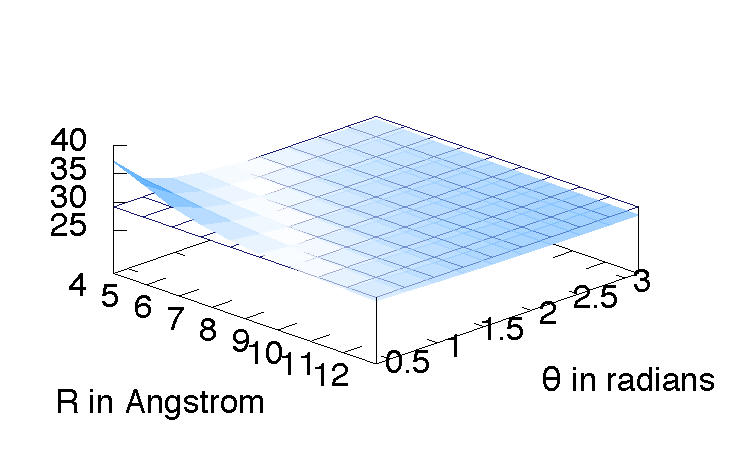
\includegraphics[scale=0.8]{pics/ArXeXe12_12_surf.pdf}
 \caption{Energy hyper surface of the doubly ionized
          ArXe5p$_{1/2}^{-1}$Xe5p$_{1/2}^{-1}$ (light blue surface) and the ionization
          potential of the Ar3s$^{-1}$ initial state with \unit[29.2]{eV}
          (dark blue grid). $Q$ is constant, whereas $R$ and the angle $\theta$
          (see figure \ref{}) are varied. This ETMD3 channel is open for
          structures where
          the final state energy is lower than the initial state energy.}
 \label{figure:ArXe2_geom_energy}
\end{figure}

At a hypothetical very small angle $\theta$ and $R\approx Q$, the channel closes.
In this example those geometries are mostly unrealistic, because the two xenon
atoms would be closer than in a neutral Xe dimer, but in other systems
channel closings due to the geometry are to be expected.


\subsection{Geometry Dependence of the ETMD3 Decay Rates}
%\subsubsection{Distance Dependencies of ETMD Decay Rates}
The decay rate also crucially depends on the geometry of the triple.
From eq. (\ref{reltheolifetimeetmd_exp}) the $R$ dependency is
easily interpreted as being
$\Gamma \propto R^{-6}$ corresponding to the energy transfer mainly being
caused by a dipole-dipole interaction. The dependency of $Q$ is implicitely
included in the transition dipole moments. These depend on the overlap
between the two atoms of the electron transfer, which decreases exponentially
with $Q$.



%\subsubsection{Angle Dependencies of ETMD Decay Rates}
The angular part of equation (\ref{reltheolifetimeetmd_exp}) can
be reformulated using
the equivalence of transitions in $\tilde{x}$ and $\tilde{y}$ direction to
yield

\begin{equation}
  \Gamma_i \propto 2 \left( |<\tilde{D}_{z}>|^2 (1+\cos^2\alpha)
                           + |<\tilde{D}_x>|^2 (2+ \sin^2\alpha) \right)
\end{equation}

The decay widths corresponding to electron transfers from orbitals
oriented along ($\tilde{z}$) and perpendicular to the internuclear axis ($\tilde{x}$)
are illustrated separately in figure \ref{figure:etmd_angle_dir}, supposing
$|<\tilde{D}_{z}>|^2 = |<\tilde{D}_x>|^2 = 1$.
Obviously, the two different transition types add up to give the full
angular dependence of a given trimer. It has to be kept in mind that in reality
$|<\tilde{D}_{z}>|^2$ is about an order of magnitude larger than
$|<\tilde{D}_{x}>|^2$.

\begin{figure}[th]
 \centering
 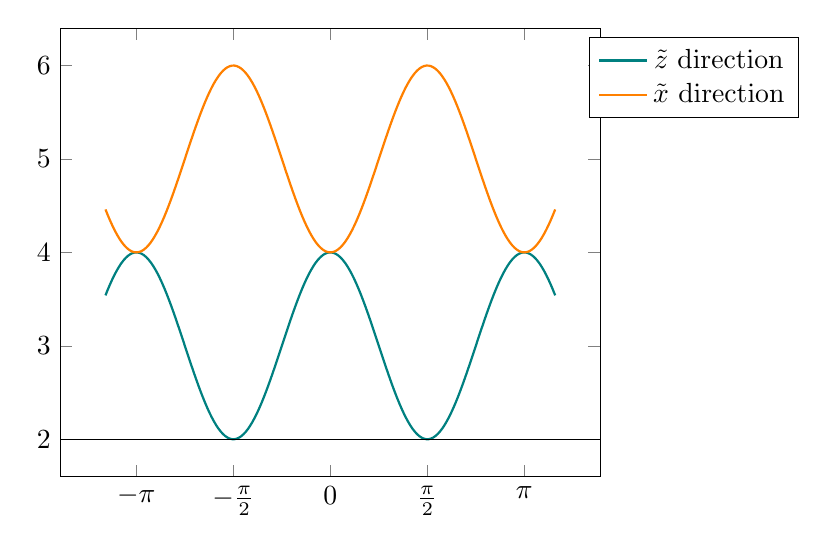
\begin{tikzpicture}
    \begin{axis}[%scale=0.8,
                 domain=-0.5-pi:0.5+pi,
                 samples = 200,
                 xtick={-3.14159,-1.57089,...,3.14159},
                 xticklabels={$-\pi$,$-\frac \pi 2$,0,$\frac \pi 2$,$\pi$},
                 cycle list name = exotic,
                 legend style={anchor= north west}
                 ]
%    \foreach \q in {0.00,0.05,0.10,0.20,0.50}{
%      \addplot+[mark = none,
%               thick
%               ]
%               {4*\q + 2 + 2*cos(deg(x))^2 + 2*\q*sin(deg(x))^2}; 
%      \addlegendentryexpanded{$q=\q$}
%               }
      \addplot+[
                mark = none,
                thick
               ]
               {2*(1+cos(deg(x))^2)};
      \addlegendentry{$\tilde{z}$ direction};
      \addplot+[
                mark = none,
                thick
               ]
               {2*(2+sin(deg(x))^2)};
      \addlegendentry{$\tilde{x}$ direction};
      \draw[] (axis cs:\pgfkeysvalueof{/pgfplots/xmin},2) -- (axis cs:\pgfkeysvalueof{/pgfplots/xmax},2);
    \end{axis}
\end{tikzpicture}

 \caption{Angle dependence of the ETMD3 decay widths for electron transfers
          along the internuclear axis $\tilde{z}$ of subsystem $S_1$ and perpendicular
          to the internuclear axis $\tilde{x}$.}
 \label{figure:etmd_angle_dir}
\end{figure}

For a more realistic picture
consider the distances $R$ and $Q$ as defined in figure \ref{etmd_geom_pspic}
to be constant and the ratio between the transition dipole moments
in the $\tilde{z}$ and the $\tilde{x}$ direction
$q=\frac{|<\tilde{D}_x>|^2}{|<\tilde{D}_z>|^2}$ to be fixed to some number.
In this case the decay width for each $M_{AB}'$ has the angular dependence

\begin{align}
 \Gamma_i &\propto \left( 2q |<\tilde{D}_{z}>|^2 +
                  (4+2q)|<\tilde{D}_{z}>|^2 \cos^2\alpha +
                  (2+4q)|<\tilde{D}_{z}>|^2 \sin^2\alpha \right) \\
          &\propto 4q + 2 + 2 \cos^2\alpha + 2q \sin^2\alpha .
\end{align}

\begin{figure}[h]
 \centering
 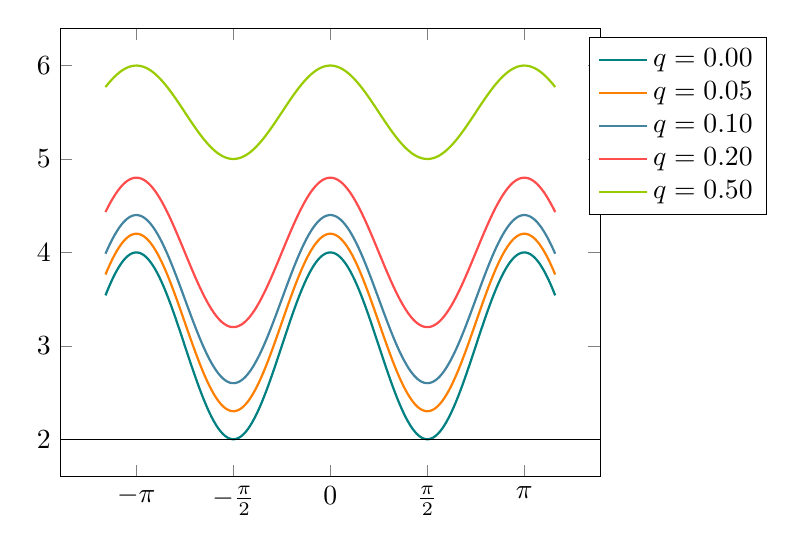
\begin{tikzpicture}
    \begin{axis}[%scale=0.8,
                 domain=-0.5-pi:0.5+pi,
                 samples = 200,
                 xtick={-3.14159,-1.57089,...,3.14159},
                 xticklabels={$-\pi$,$-\frac \pi 2$,0,$\frac \pi 2$,$\pi$},
                 cycle list name = exotic,
                 legend style={anchor= north west}
                 ]
    \foreach \q in {0.00,0.05,0.10,0.20,0.50}{
      \addplot+[mark = none,
               thick
               ]
               {4*\q + 2 + 2*cos(deg(x))^2 + 2*\q*sin(deg(x))^2}; 
      \addlegendentryexpanded{$q=\q$}
               }
      \draw[] (axis cs:\pgfkeysvalueof{/pgfplots/xmin},2) -- (axis cs:\pgfkeysvalueof{/pgfplots/xmax},2);
    \end{axis}
\end{tikzpicture}

 \caption{Angular dependence of the \ac{ETMD}3 decay width for electron transfers
          both along and perpendicular to the internuclear axis of subsystem $S_1$.
          Different values of $q=\frac{|<\tilde{D}_x>|^2}{|<\tilde{D}_z>|^2}$.}
 \label{figure:etmd_angle}
\end{figure}



It is an oscillating function with maxima at even multiples of $\frac \pi 2$
and minima at uneven multiples at $\frac \pi 2$ as shown in figure
\ref{figure:etmd_angle}.


In a real system, an energy transfer between
two dipoles is most efficient, if they are aligned in one direction.
Within a dimer the most efficient electron transfer results in a
dipole aligned along the bonding axis and hence $q<1$. A typical
value of $q$ would be $\frac 1{10}$. In the 
case of $q$ approaching 0, the angular part of
the decay width
approaches a shifted $2\cos^2 \alpha$ with maxima at even multiples of $\frac \pi2$
and minima at uneven multiples of $\frac \pi2$ with values between
$4$ and $2$.
Therefore, for typical numbers of $q$ the energy transfer
to an atom on the same axis ($\alpha = 0,\pi$), corresponding
to a linear arrangement, is preferred.

The previous discussions are based on the decay of one specific atom
being the electron donor and another atom being the electron emitter.
In reality both atoms can be donor als well as emitter while the energy
of the resulting final state stays the same. For both bond lengths between the
two atoms ionized in the final state and
initially ionized atom being the same, both contribute the same amount
to the total decay rate. With one of the atoms ionized in the final state
being further apart, its probability in donating the vacancy filling electron
decreases exponentially and can hence be neglected.

%\afterpage{\clearpage}
\begin{figure}[ht]
 \centering
 \begin{tikzpicture}
    \begin{axis}[scale = 0.8,
                 domain= 20:180,
                 y domain=4.0:15,
                 xtick={30,60,...,180},
                 cycle list name = exotic,
                 xlabel = {$\theta$},
                 ylabel = {$R$ [\AA]},
                 zlabel = {$\Gamma$ [eV]},
                 title = {ArXe5p$_{3/2}^{-1}$Xe5p$_{3/2}^{-1}$},
                 %view={0}{0}
                 view={230}{10}
                 ]
    \addplot3[surf,
             z buffer=sort
             ]
             table[
             x expr=\thisrowno{1},
             y expr=\thisrowno{0},
             z expr=\thisrowno{2}
             ]
             {data/ArXe2_etmd_surf.dat};
    \end{axis}
\end{tikzpicture}

 \begin{tikzpicture}
    \begin{axis}[scale = 0.8,
                 domain= 20:180,
                 y domain=4.0:15,
                 xtick={30,60,...,180},
                 cycle list name = exotic,
                 xlabel = {$\theta$ [$^{\circ}$]},
                 ylabel = {$R$ [\AA]},
                 zlabel = {$\Gamma$ [eV]},
                 title = {ArXe5p$_{3/2}^{-1}$Xe5p$_{1/2}^{-1}$},
                 %view={0}{0}
                 view={230}{10}
                 ]
    \addplot3[surf,
             z buffer=sort
             ]
             table[
             x expr=\thisrowno{1},
             y expr=\thisrowno{0},
             z expr=\thisrowno{3}
             ]
             {data/ArXe2_etmd_surf.dat};
    \end{axis}
\end{tikzpicture}
\\
 \begin{tikzpicture}
    \begin{axis}[scale = 0.8,
                 domain= 20:180,
                 y domain=4.0:15,
                 xtick={30,60,...,180},
                 cycle list name = exotic,
                 xlabel = {$\theta$},
                 ylabel = {$R$ [\AA]},
                 zlabel = {$\Gamma$ [eV]},
                 title = {ArXe5p$_{1/2}^{-1}$Xe5p$_{3/2}^{-1}$},
                 %view={0}{0}
                 view={230}{10}
                 ]
    \addplot3[surf,
             z buffer=sort
             ]
             table[
             x expr=\thisrowno{1},
             y expr=\thisrowno{0},
             z expr=\thisrowno{4}
             ]
             {data/ArXe2_etmd_surf.dat};
    \end{axis}
\end{tikzpicture}

 \begin{tikzpicture}
    \begin{axis}[scale = 0.8,
                 domain= 20:180,
                 y domain=4.0:15,
                 xtick={30,60,...,180},
                 cycle list name = exotic,
                 xlabel = {$\theta$},
                 ylabel = {$R$ [\AA]},
                 zlabel = {$\Gamma$ [eV]},
                 title = {ArXe5p$_{1/2}^{-1}$Xe5p$_{1/2}^{-1}$},
                 %view={0}{0}
                 view={230}{10}
                 ]
    \addplot3[surf,
             z buffer=sort
             ]
             table[
             x expr=\thisrowno{1},
             y expr=\thisrowno{0},
             z expr=\thisrowno{5}
             ]
             {data/ArXe2_etmd_surf.dat};
    \end{axis}
\end{tikzpicture}

 \caption{\ac{ETMD}3 decay widths $\Gamma$ hyper surfaces for an ArXe$_2$ trimer.
          The four electronic decay channels are shown separately.}
 \label{figure:ArXe2_etmd_geom_gamma}
\end{figure}


Combining both the view on the energetic accessibility of the decay
channels and the decay widths results in the pictures in
figure \ref{figure:ArXe2_etmd_geom_gamma}.
Here the geometry dependence of the decay width for the case of the four ArXe$_2$
channels is shown summing the decay widths of the two possible geometric combinations
of the triple.
The numbers were obtained by \ac{HARDRoC} using the
asymptotic formula (\ref{reltheolifetimeetmd_exp}) with redefined
$R$ and $\theta$. Here $Q=\unit[4.04]{\AA}$ is chosen constant
to the internuclear distance of the neutral ArXe dimer while $R$ and $\theta$
are varied. The plots display the channel closing for very small Xe-Xe distances
and the $R^{-6}$ behaviour as well as the expected angle dependence explicitely
shown in figure \ref{figure:etmd_angle}. Implicitly the exponential decrease
of the decay width is shown by one of the two triple combinations in the trimer
showing a contribution only at small internuclear distances.

The decay widths of the four different decay channels shown in
figure \ref{figure:ArXe2_etmd_geom_gamma} can be summed up to yield
the total decay width of the ArXe$_2$ trimer as illustrated in figure
\ref{figure:ArXe2_etmd_geom_gamma_total}.

\begin{figure}[h]
 \centering
 \begin{tikzpicture}
    \begin{axis}[scale = 0.8,
                 domain= 20:180,
                 y domain=4.0:15,
                 xtick={30,60,...,180},
                 cycle list name = exotic,
                 xlabel = {$\theta$},
                 ylabel = {$R$ [\AA]},
                 zlabel = {$\Gamma$ [eV]},
                 title = {Total decay width of the ArXe5p$^{-1}$Xe5p$^{-1}$},
                 %view={0}{0}
                 view={230}{10}
                 ]
    \addplot3[surf,
             z buffer=sort
             ]
             table[
             x expr=\thisrowno{1},
             y expr=\thisrowno{0},
             z expr=\thisrowno{6}
             ]
             {data/ArXe2_etmd_surf.dat};
    \end{axis}
\end{tikzpicture}

 \caption{Sum over the decay widths of all four channels, illustrated
          separately in figure \ref{figure:ArXe2_etmd_geom_gamma}.
          The opening of channels at different angles $\theta$ and
          internuclear distances $R$ are to be seen at the spikes.}
 \label{figure:ArXe2_etmd_geom_gamma_total}
\end{figure}

Also here the $R^{-6}$ dependence is observed but the dependency
of the angle $\theta$ shows spikes. These changes are due to the channel
closing. For a large angle $\theta$ all channels are open. Imagine a linear
trimer, which now starts bending. The closer
the two xenon atoms get, the more the two positive charges in the final
state repell each other. At one point the atoms are so close, that the
ArXe5p$_{1/2}^{-1}$Xe5p$_{1/2}^{-1}$ channel being highest in energy
is no longer energetically accessible. Bending further, first the
ArXe5p$_{3/2}^{-1}$Xe5p$_{1/2}^{-1}$ and the
ArXe5p$_{1/2}^{-1}$Xe5p$_{1/2}^{-1}$ channels, being equal in energy,
close. In the illustrated angle range the ArXe5p$_{3/2}^{-1}$Xe5p$_{3/2}^{-1}$
channel does not close.


\section{Influence of the Coordinate System Choice} \label{section:coord_choice}
In figure \ref{etmd_geom_pspic} a coordinate
system was chosen to describe the
triatomic system $ABC$. The distance $Q$ between the two atoms involved
in the electron transfer is reasonably defined. However, where the
center of the oscillating dipole moment of subsystem $S_1$ is located, can
not unambigously be defined. Most
probable it is somewhere between the atoms $A$ and $B$.
The coordinates were chosen as illustrated in the left panel of figure
\ref{figure:coord_etmd_comparison} with the distance $R$ of the energy transfer
anchoraged at the initially ionized atom $A$. This choice is convenient for
the calculation of the decay widths of large system, since for triples
consisting of atoms at larger distances the possibility of the anchorage to
coincide with atom $C$ is avoided.
Another possible choice would be some point between the atoms $A$ and $B$ as
illustrated in the right panel of figure \ref{figure:coord_etmd_comparison}.

\begin{figure}
 \centering
 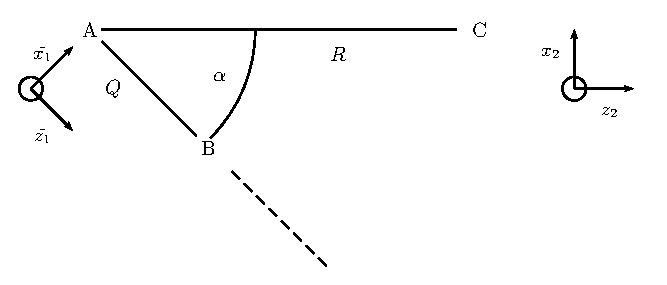
\includegraphics[scale=0.6]{pics/coord_etmd_alt_pspic.eps}
 \hfill
 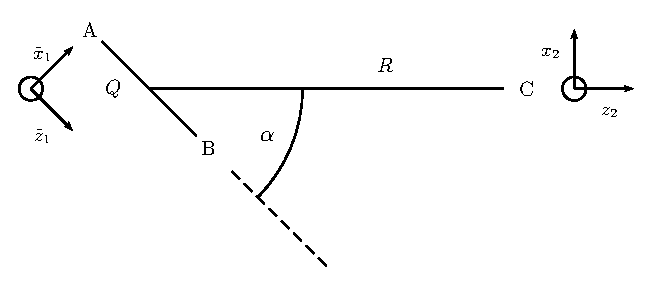
\includegraphics[scale=0.6]{pics/coord_etmd_pspic.eps}
 \caption{Two different set of Jacobi coordinates for the description of a triple
          $ABC$ (compare figure \ref{etmd_geom_pspic}).
          In the left figure the distance of the energy transfer originates
          at the initially ionized atom $A$, while in the right panel the
          energy transfer distance is defined with respect to some
          point between atoms $A$ and $B$. The right choice might be
          physically more precise, even though it it unknown, how to choose
          the anchorage point. The left set of coordinates is preferable
          in the modelling of cluster structures.}
 \label{figure:coord_etmd_comparison}
\end{figure}

For the following discussion we will therefore refer to two sets
of coordinates of maximum deviation with origins residing in atoms
$A$ and $B$ with subscripts $A$ and $B$.

We assume that we have two constant distances $R_{A}$ and $R_B$
where either of these distances is larger than or equal to $Q$.
In this case the maximum and minimum of the ratio between the two
corresponding decay rates $\frac{\Gamma_{A}}{\Gamma_B}$ will occur
in the case of $\alpha = 0,\pi$ and $R_B = \frac 12 R_{A} = Q$
and $R_B = 2 R_{A} = 2Q$, respectively.

\begin{figure}[h]
 \centering
    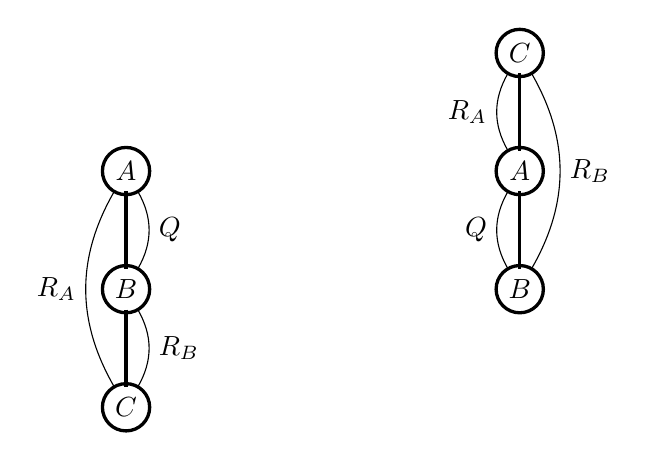
\begin{tikzpicture}[scale=1.0,>=stealth]
%       \draw [help lines] (0,0) grid (10,7);
       
       \draw [very thick] (2,4) circle (0.3)
              node [name=A] {$A$};
       \draw [very thick] (2,2.5) circle (0.3)
              node [name=B] {$B$};
       \draw [very thick] (2,1) circle (0.3)
              node [name=C] {$C$};
       \draw [very thick] (A) -- (B);
       \draw [very thick] (B) -- (C);
       \path (A) edge [bend left] node [right] {$Q$} (B)
             (B) edge [bend left] node [right] {$R_B$} (C)	
             (A) edge [bend right] node [left] {$R_A$} (C);

    \begin{scope}[xshift=5cm]
       \draw [very thick] (2,4) circle (0.3)
              node [name=A] {$A$};
       \draw [very thick] (2,2.5) circle (0.3)
              node [name=B] {$B$};
       \draw [very thick] (2,5.5) circle (0.3)
              node [name=C] {$C$};
       \draw [very thick] (A) -- (B);
       \draw [very thick] (A) -- (C);
       \path (A) edge [bend right] node [left] {$Q$} (B)
             (B) edge [bend right] node [right] {$R_B$} (C)	
             (A) edge [bend left] node [left] {$R_A$} (C);
    \end{scope}

   \end{tikzpicture}

 \caption{Illustration of two geometry parameter sets, which lead
          to the largest possible deviation of the ETMD decay width.}
 \label{}
\end{figure}

\begin{equation}
\text{minimum: } \frac{\Gamma_{A}}{\Gamma_B}= \frac{1}{64} = \frac{1}{2^6} \quad ,\quad
\text{maximum: } \frac{\Gamma_{A}}{\Gamma_B}= \frac{64}{1}
\end{equation}

From this we conclude, that the absolute numbers of calculated ETMD
decay widths are obviously error-prone. In the worst case the uncertainty
is given by factors $\frac{1}{64}$ or $\frac{64}{1}$.
In reality these worst cases will rarely be observed, since it on
the one hand is very unlikely to find two atoms at exactly the same place
and on the other hand ETMD preferably occurs at interfaces, which leads
to preferred angles higher than 0 and below $\pi$.
Additionally the larger the difference between $Q$ and $R$ is, the
smaller this effect is going to be.


